\chapter{Experimental Dataset}
Data is the core in data-driven or machine learning based applications. This chapter describes the dataset and the experimental procedure used in this research. First, the cyclic fatigue testing was conducted till the rupture of a material to acquire the fatigue characteristics of a material such as S-N curve. Second, to mimic the scenarios in the remanufacturing industry, interrupted fatigue testing was utilized to produce samples at different fatigue level as simulated end-of-life products. Linear and nonlinear ultrasound measurements are used to evaluate the fatigue damage of those samples stopped at the predetermined number of cycles in the interrupted fatigue testing. Besides, the residual stress and full-width-at-half-maximum data from X-ray diffraction are also presented.

\section{Life cycle fatigue testing}
The life cycle fatigue testing aims to collect the fatigue life data to comprehensively understand the fatigue behavior of our targeted material. The fatigue life of a material is defined as the total number of cycles that a material can sustain under a specified loading condition. In order to develope the S-N curve of a material, the material is tested at different loading stress amplitudes, and the fatigue test is repeated multiple times for each loading stress amplitude to account for the variance of fatigue life.

The fatigue testing is led by Prof. Jingjing Li's group at the Penn State University. The targeted material in this research is 5052-H32 aluminum alloy. Figure \ref{fig: fatigue testing setup} shows the dimension of the specimen and the fatigue testing machine in this research. Three loading amplitudes , 11.7, 12.7, and 14.7 kN in the cyclic fatigue testing are selected to develop the S-N curve shown in Figure \ref{fig: raw sn curve}. 

\begin{figure}[tb]
  \begin{subfigure}[t]{0.50\linewidth}
    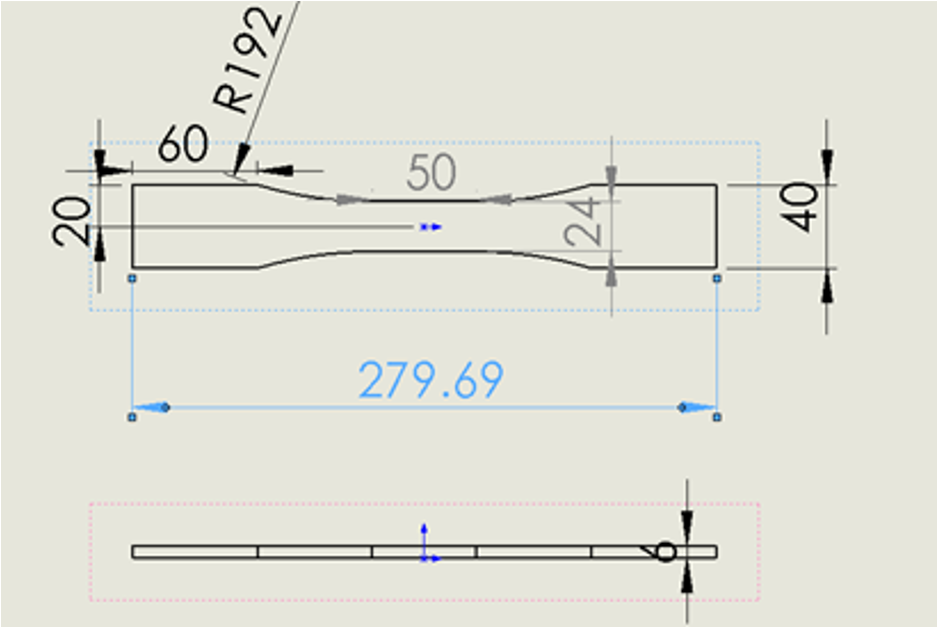
\includegraphics[height=0.7\textwidth]{fig/specimen_dim.png}
    \caption{The 2-D illustration of the 5052-H32 aluminum alloy specimen}
    \label{fig: specimen dim}
  \end{subfigure}
  \begin{subfigure}[t]{0.50\linewidth}
    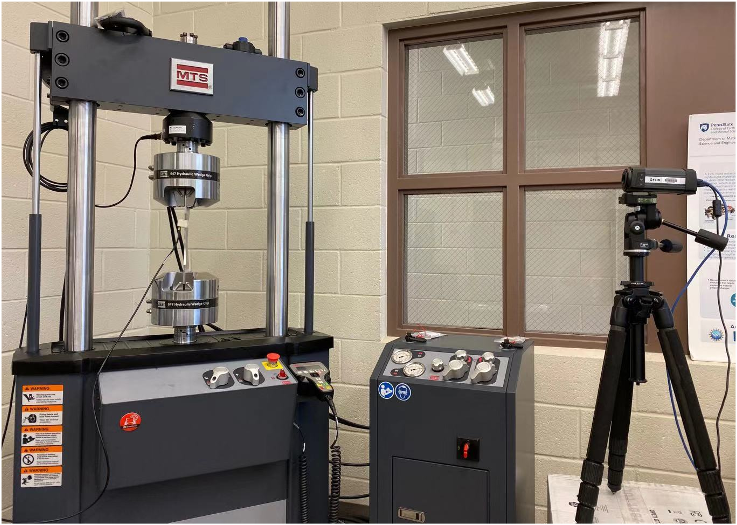
\includegraphics[height=0.7\textwidth]{fig/fatigue_testing_machine.png}
    \caption{MTS 100KN Landmark fatigue testing system at Prof. Jingjing li's lab}
    \label{fig: fatigue testing machine}
  \end{subfigure}

  \caption{Life cycle fatigue testing setup}
  \label{fig: fatigue testing setup}
\end{figure}

\begin{figure}[tb]
  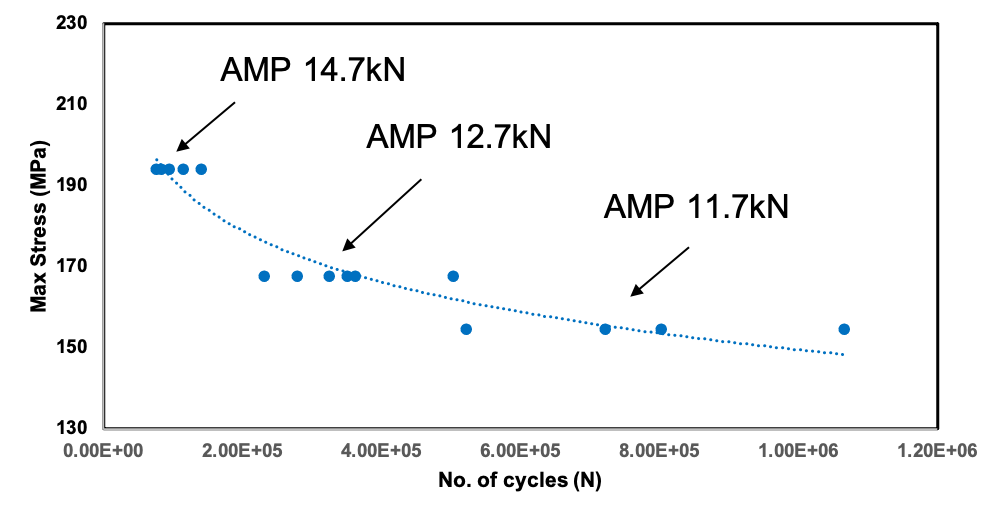
\includegraphics[width=\linewidth]{fig/sn_curve.png}
  \caption{Development of the S-N curve of 5052-H32 aluminum alloy}
  \label{fig: raw sn curve}
\end{figure}

\section{Interrupted fatigue testing}

\section{Linear ultrasound measurement}
\section{Nonlinear ultrasound measurement}
\section{X-ray diffraction measurement}
